\documentclass{standalone}
\usepackage{tikz}
\usetikzlibrary{arrows.meta, positioning, quotes}
\begin{document}
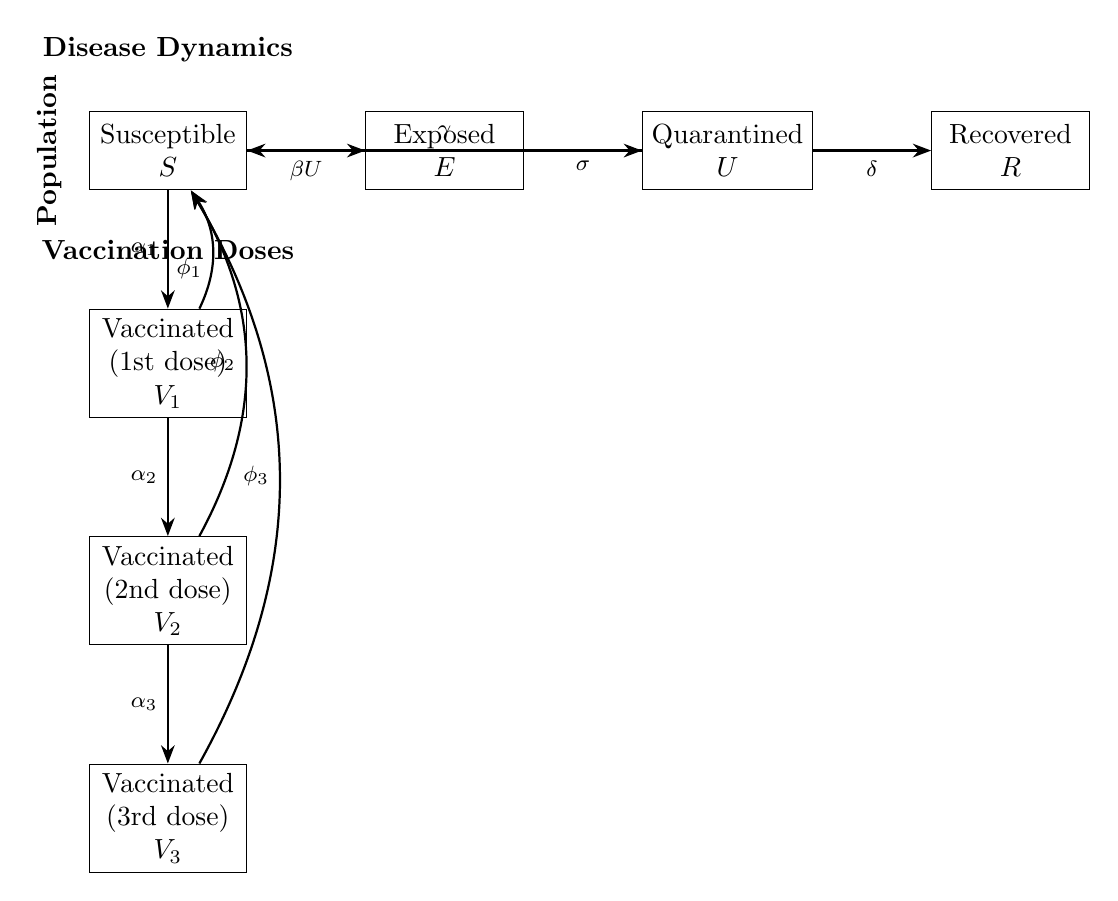
\begin{tikzpicture}[
    compartment/.style={draw, rectangle, minimum width=2cm, minimum height=1cm, align=center},
    arrow/.style={-Stealth, thick},
    every edge quotes/.style={auto=right, font=\footnotesize},
    node distance=1.5cm and 1.5cm
]
    % Compartments
    \node[compartment] (S) {Susceptible\\$S$};
    \node[compartment, right=of S] (E) {Exposed\\$E$};
    \node[compartment, right=of E] (U) {Quarantined\\$U$};
    \node[compartment, right=of U] (R) {Recovered\\$R$};
    
    \node[compartment, below=of S] (V1) {Vaccinated\\(1st dose)\\$V_1$};
    \node[compartment, below=of V1] (V2) {Vaccinated\\(2nd dose)\\$V_2$};
    \node[compartment, below=of V2] (V3) {Vaccinated\\(3rd dose)\\$V_3$};
    
    % Transitions
    \draw[arrow] (S) edge["$\beta U$"] (E);
    \draw[arrow] (E) edge["$\sigma$"] (U);
    \draw[arrow] (U) edge["$\delta$"] (R);
    \draw[arrow] (U) edge["$\gamma$"] (S);
    
    \draw[arrow] (S) edge["$\alpha_1$"] (V1);
    \draw[arrow] (V1) edge["$\alpha_2$"] (V2);
    \draw[arrow] (V2) edge["$\alpha_3$"] (V3);
    
    \draw[arrow] (V1) edge[bend right, "$\phi_1$"'] (S);
    \draw[arrow] (V2) edge[bend right, "$\phi_2$"'] (S);
    \draw[arrow] (V3) edge[bend right, "$\phi_3$"'] (S);
    
    % Annotations
    \node[above=0.5cm of S] {\textbf{Disease Dynamics}};
    \node[above=0.5cm of V1] {\textbf{Vaccination Doses}};
    \node[left=0.5cm of S, rotate=90, anchor=center] {\textbf{Population}};
\end{tikzpicture}
\end{document}